\chapter{Process Analysis}

As this project have mainly been focused on learning new topics on our own, it is important to also talk about the outcome of the specialization period. This chapter will go over the goals of the project and whether or not we feel these goals have been achieved.

\section{Project Planning}
At the beginning of the semester we were to make a specialization description which contain goals we want to achieve doing the specialization period. My goal was to analyze and look for opportunities for making IRLVRMMO Games more interactive, as well as cooperative and competitive in a similar way to modern pc games, and what technologies could be used to make such games.

We were also to create a schedule that we had to follow through the project, that can be seen in \figref{fig:InitPlan}.

\begin{figure}[H]
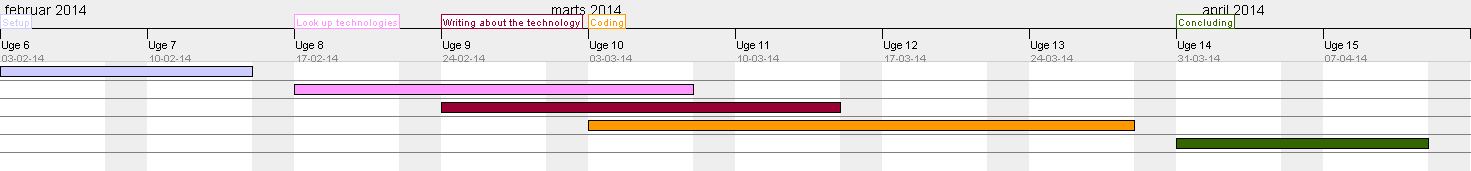
\includegraphics[width=1\linewidth]{img/InitPlan}
\centering
\caption{The initialized schedule}
\label{fig:InitPlan}
\end{figure}

However, due to a fast start and lots of course related work in the middle of the semester, as well as the coding took longer than expected, some changes were made to make up for both the very productive first weeks and the busy weeks in the middle of the semester. The changed schedule can be seen In \figref{fig:actPlan}.

\begin{figure}[H]
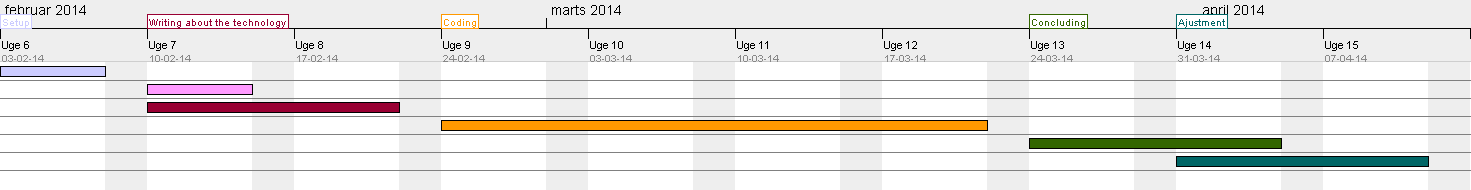
\includegraphics[width=1\linewidth]{img/actPlan}
\centering
\caption{The initialized schedule}
\label{fig:actPlan}
\end{figure}

As most of the setup and planning was done before the semester started and the first few weeks didn't have much course related work, we had all the setup and introducing chapters done much faster than planned. On the other hand the coding took longer than first expected, as there was more work those weeks related to courses, and it took us longer to get to know the android SDK and set it up probably.


\section{Work Process}

Our goal was to attend every course in game development and android development to get the most needed support and knowledge on our topic, but none of the courses touched any relating topics. Additional research was required, and our plan was to find video tutorials and scientific articles or papers and blog post from reliable sources to get information about the topic. We did not find reliable sources on every subtopics related to our main topic, which is probably due to the fact that this topic is very new.

We took focus in a paper explaining the ideas and technologies that can be used to implement such game but we also made a working prototype, of an online game played in the real world. This was done to get an overall idea over how the technology behind works, and how it can be used in practice.

Our work plan was planed to be about 8 hours work each day/40 hours a week (this including courses and work related to those) but we ended up using slightly less time some days, and other days slightly more, but being in control of our own time and studies have been great rather than relying on others to teach us.

We did not have a plan or any knowledge about what the product should be like or how it should work, and even some subtopics was very new to us. Even Java and android was new to us, and therefore we went with the "trial and error" and "Hack and slash" way of developing, where we slowly made small parts of the program work, tested it, and tried to understand how everything worked, and when added a little more code, and so on, until we had our working prototype. We primarily made the parts by finding some articles or forum talking about how it worked and then putting it together to a single part of the system and then adding a new part to it and make them communicate, e.g. we first added the Google map overlay, then added GPS input to it, then icons and later on network communication. This may have been a slower way of learning and developing than normal, but taking into account that this topic is still new, and somewhat untouched, may lead to believing that slow and safe is the way to go if you really want most out of such topic.


\section{Usage of Courses}

Throughout the Specialization period we planed on attending every course in game development and Android development as these topics seemed important to the learning outcome on the Specialization, but most of the topics didn't touch key features related to our work. Android did only did touch some general areas of using location services and sensors which was related to my project, but most topic was however useful and could surely be used in future projects.


\section{Learning Outcome}

As previously mentioned our goal was to analyze and look for opportunities for making IRLVRMMO and how they could mimic modern pc games, and what technologies could be used to make such games.

Since the making of MMOs can take years of development we have identified some key features to work on, that was possible to complete within the given timespan of 10 weeks. Some ideas have been explained to give a general knowledge about what would have been a better solution, but there have been prioritized to what should be implemented and what decisions have been made on the project to made the finished product.

The learning outcome for this project have been enormous, but not every goal have been reached as due to the time limit. The project is not in anyway optimized for massive multiplayer online gaming but instead made for private online play, where some friends could potentially play together. As mentioned in chapter \ref{cha:MMO} Client-side prediction would have been an important implementation for the game to work with hundreds of clients connected simultaneously. The game could be expanded and have this implemented at a later stage or if there had been more time to implement it probably. It can also be discussed how well the cooperative and competitive part is involved in the game, but team work may be needed by both teams, on games where many players would play at once.

There has been a lot of study and great learning outcomes in this project. Learning the Java programming language and android SDKs has been a challenge since it is the first larger project it has been used for, but we now feel much more comfortable using it and will probably use it in future projects. In the beginning of the project we also did a lot of research on how the phones hardware could be used for gaming purposes, e.g. using the phone's gyroscope to simulate raycast or tracelines but was not implemented due to limitations mentioned in chapter \ref{cha:FutureWork}. We have also scratched the surface of how to make online games using socket programming and how these games can potentially mimic other real games, and furthermore use the real world as the game world for these games, and thereby creating a virtual world within the real world. We have mentioned Client-side prediction and how this is used in other multiplayer games and how it could help improve the game latency.


\section{Project Conclusion}

This project have taken much focus in self study, and learning on you own which we have been happy for. There have been a great amount of time for us to learn and study our topic and done it the way we feel we would learn it best. We are very excited for this kind of study and would without doubt love to have the possibility to work like this in an other semester.

Our learning outcome for this semester feels like it have been much bigger and better than it have in other semester, which could be either true or purely due to the fact that the topic is something we are interested in.

One major drawback of this semester was the amount of supervision and needs of explanations of the learning methods. We felt like this was taking up a larger amount of time that could have been used on improving the final product or have learned even more on the topics studied. Our thoughts is that the final product should speak for it self and should have the potentials to show if the intended learning outcome have been accomplished.